\chapter{Analyse}

\section{Aufgabe und Ziel}
Diesen punkt streichen!

\section{Ist Situation}
In der Vorgängerarbeit \enquote{Cygnet} von Stefan Rohner und Marco Tanner
<TODO: Ref> wurde der Policy Server \enquote{strongTNC} implementiert. Das
Produkt und die Codebasis dieser Arbeit dient als Grundlage für diese Arbeit.\\
Im Bereich des SWID Generators gibt es zur Zeit noch keine bestehenden Produkte.

\subsection{Stand der strongTNC Webapplikation} 
strongTNC ist eine Umsetzung des TNC Policy Servers, implementiert wurde dieser
als Webapp mit dem Python basierten \enquote{Django Web Framework} in Version 1.6 <TODO: Ref>.
Die Applikation bietet Unterstützung für das Verwalten von Geräten, Policies,
Enforcements und erlaubt es die Anwendung der Enforcements mittels
hierarchischer Gruppen zu steuern. Stammdaten wie Dateien oder Softwarepakete
und Messresultate können eingesehen und teilweise bearbeitet werden. Für SWID
Tags besteht derzeit keine Unterstützung, allerdings wurden bereits Views für
SWID Tags und Regids erstellt, diese haben jedoch keine Funktionalität und
dienen gewissermassen als Vorschau für zukünftige Features. \\
Im Frontend der Webapplikation wurden Bootstrap 2.3 sowie jQuery 1.9 <TODO:
Ref> eingesetzt. Grundsätzlich werden die Ansichten als \enquote{Master-Detail
View} <TODO: Ref> dargestellt.
Als Schnittstelle zur strongSwan IPsec Infrastruktur dient eine gemeinsam
genutzte SQLite <TODO: Ref> Datenbank. 

Django Webapplikationen lassen sich in Module, sogenannte \enquote{Apps},
aufteilen, diese Möglichkeit wird allerdings nicht genutzt wie man dem
Diagramm der Applikation entnehmen kann, \autoref{django-ist-diagram}. Die
Django-Models sind sehr eng an das Datenbankschema angelehnt, es ist gängig,
dass die Datenbank aus den Models generiert wird, dadurch wird die Datenbank für
den Entwickler vollständig abstrahiert. Da die Datenbank als Schnittstelle dient
und darum nicht ausschliesslich von Django verwendet wird, kann dieses Feature
nicht genutzt werden. Das Datenbankschema kann im Anhang eingesehen werden
(<TODO: Ref>)

\begin{figure}[H]
	\centering
	\includegraphics[width=\textwidth]{images/architecture/django_apps_ist}
    \caption{Monolithische Django App}
    \label{django-ist-diagram}
\end{figure}

Den Ablauf einer Messung kann man dem folgenden Sequenzdiagramm,
\autoref{architecture-sequence-diagramm}, entnehmen:
\begin{figure}[H]
	\centering
	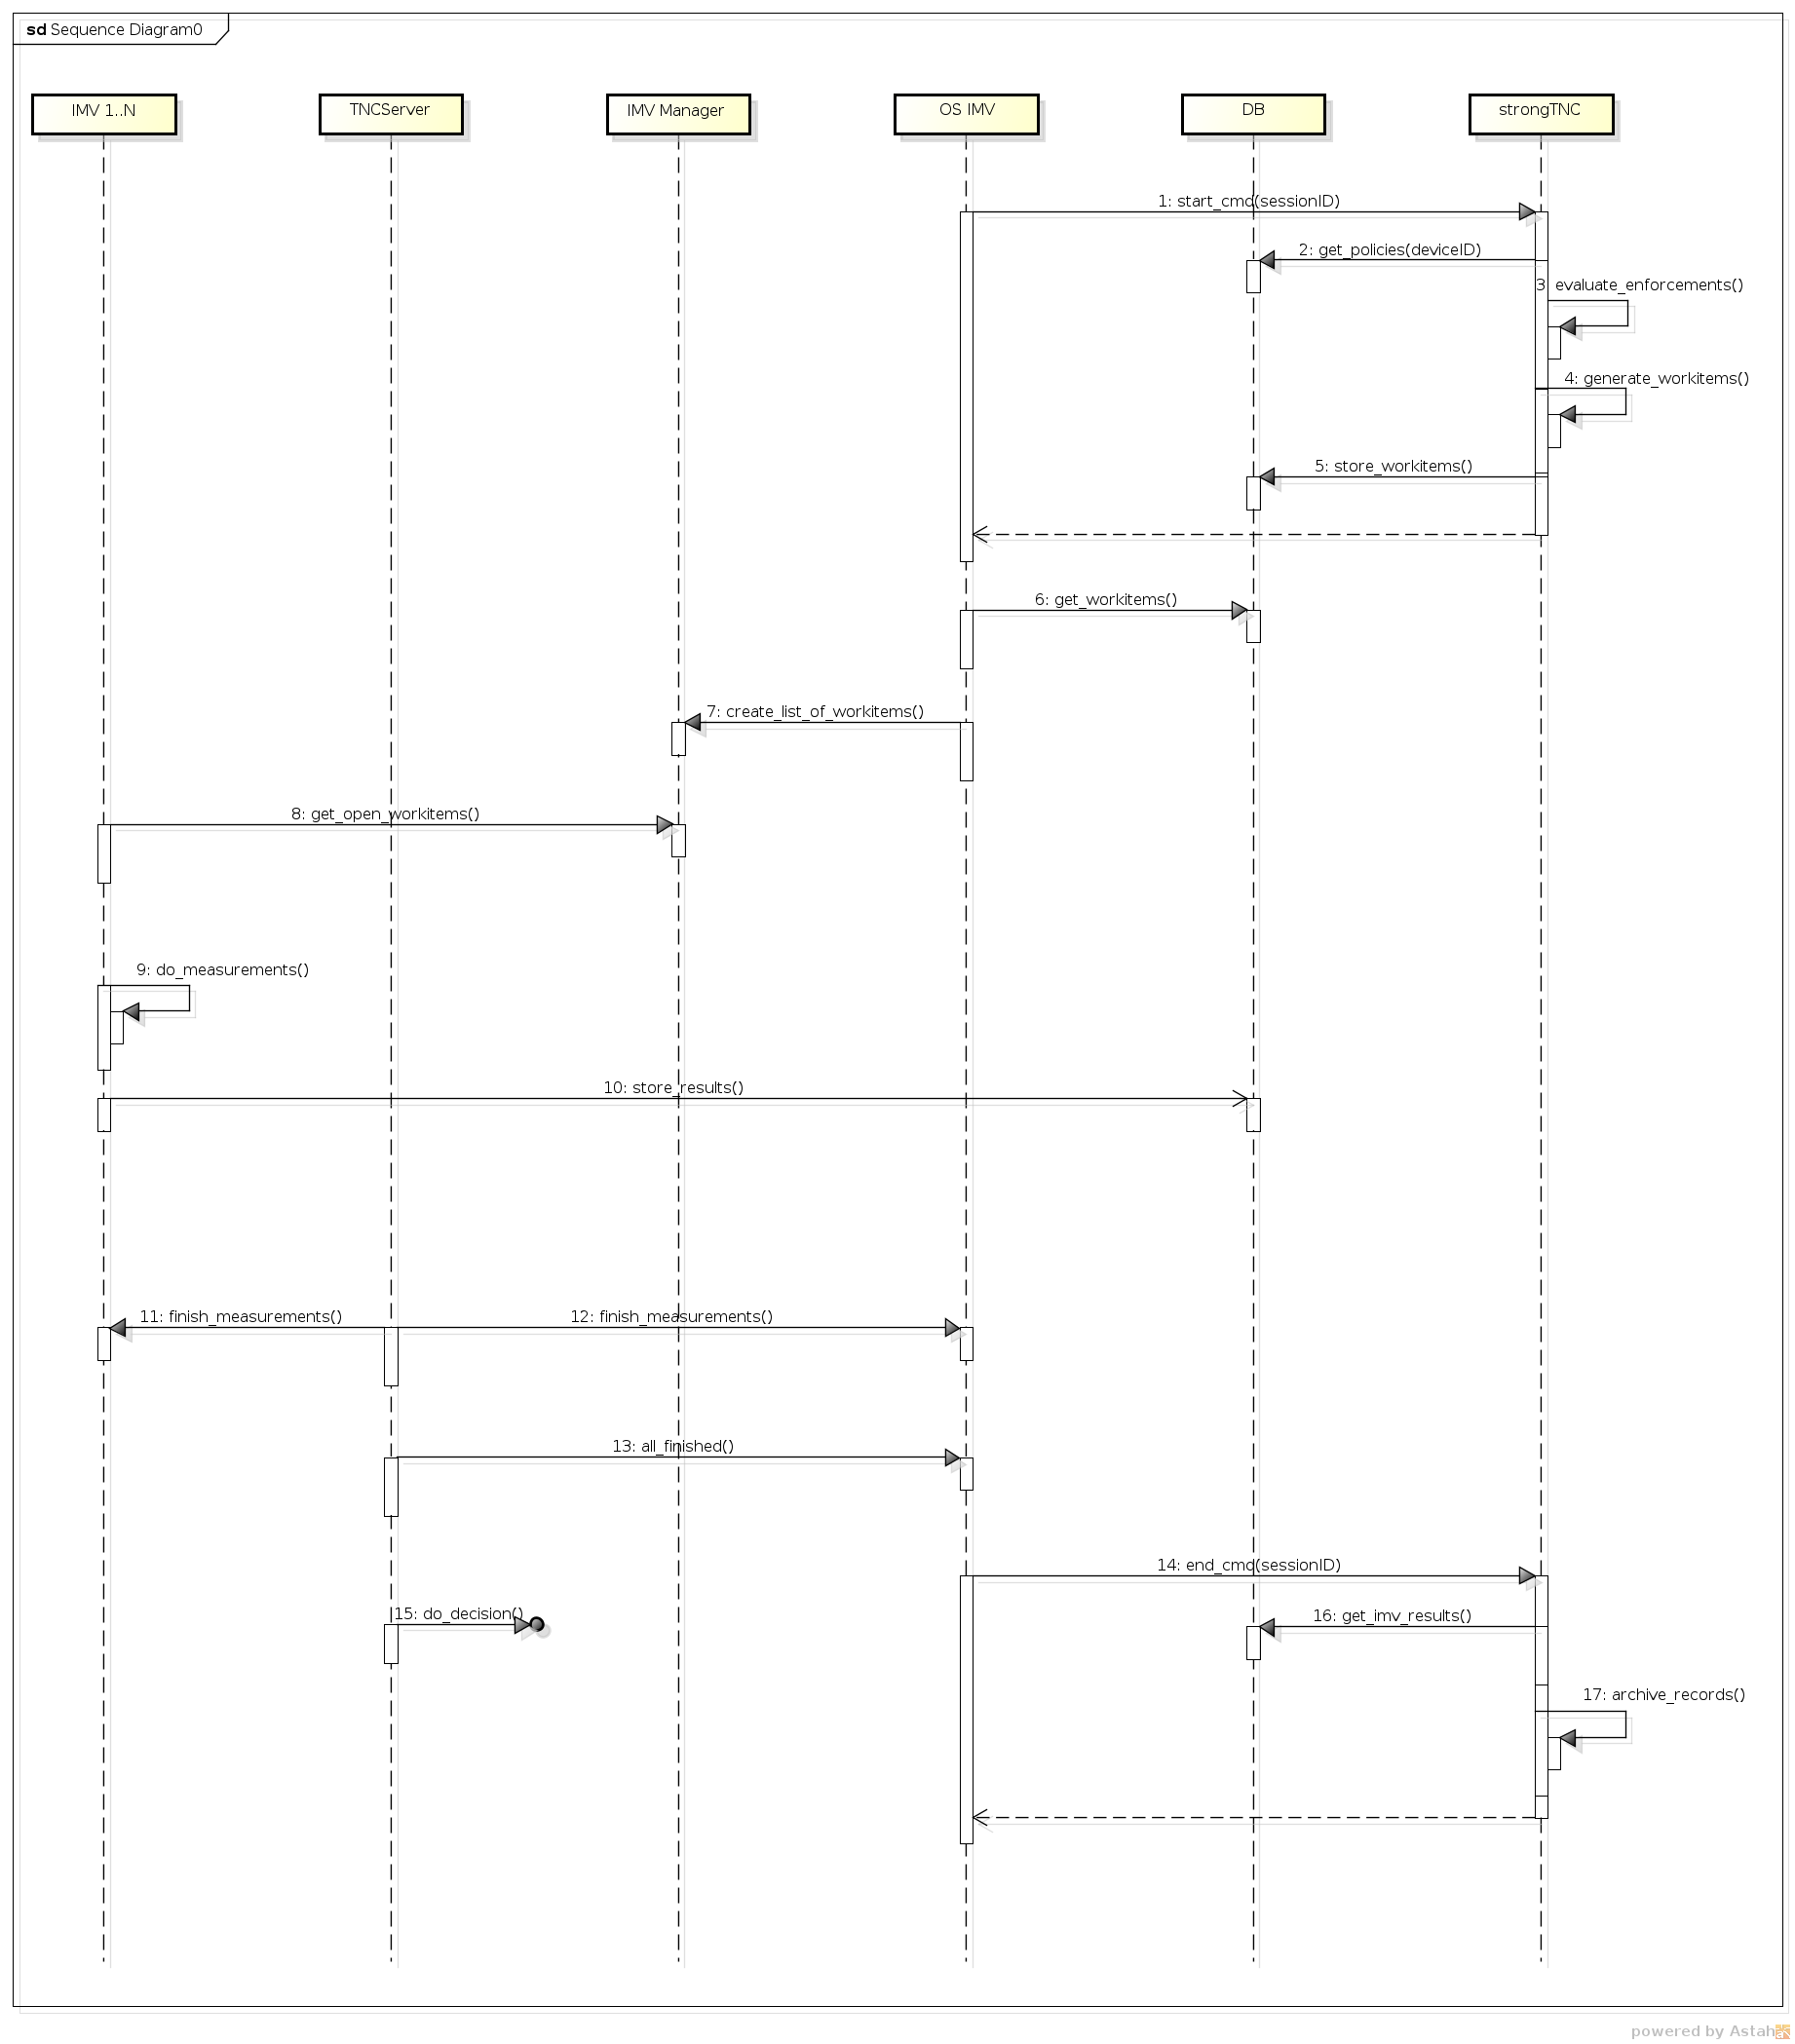
\includegraphics[width=\textwidth]{./images/architecture/architecture_sequence_diagramm-2014-03-12}
	\caption{}
	\label{architecture-sequence-diagramm}
\end{figure}

Laut dem technischen Bericht der der Vorgängerarbeit \enquote{Cygnet} <TODO:
Ref> sollen die Richtlinien des \enquote{Style Guide for Python Code} <TODO:
Ref>, genannt PEP8, eingehalten werden. Es existieren elf Unit-Tests welche den
bestehenden Python Code zu 21\% abdecken.\\


\subsubsection{Einschätzung}
\begin{description}
	\item[Ergänzungen] Es existiert noch keine Möglichkeit zur Erfassung und
	Verwaltung von SWID Tags, diese müssen im Rahmen dieser Arbeit erstellt werden.
	Die bestehenden Views können gegebenenfalls als Vorlage verwendet werden.
	
	\item[Schnittstelle] Das Verwenden einer gemeinsamen Datenbank stellt in unseren
	Augen ein Architekturproblem dar, welches dringend angegangen werden muss.
	Einerseits wird die Interoperabilität mit anderen Systemen stark eingeschränkt,
	andererseits wird die Wartbarkeit und Ausbaufähigkeit aller beteiligten
	Komponenten erschwert oder verunmöglicht. In diesem Fall wird ausserdem SQLite
	als Datenbank verwendet. SQLite ist nur bei lesendem Zugriff mehrbenutzerfähig,
	bei schreibendem Zugriff wird die Datenbank gesperrt, da eine gemeinsam
	genutzte Datenbank Mehrbenutzerbetrieb impliziert, sollte auch in diesem Bereich
	etwas unternommen werden. 
	
	\item[Benutzerschnittstelle] 
	Die Benutzeroberfläche wurde noch nicht für den Umgang mit grossen Datenmengen
	optimiert. Bei einer grossen Anzahl Objekten gibt es keinen Paging Mechanismus,
	der ein Stückweises ausliefern von Daten oder Filtern erlaubt. Beispielsweise
	kann das Inventar der Dateinamen in einem Linux System kann durchaus 40000
	Objekte umfassen. Wird die vorhandene File View aufgerufen, werden alle 40000
	Einträge angezeigt. Diesen möglichen Dimensionen wird zur Zeit noch nicht
	Rechnung getragen, und hat sich bereits beim Entwickeln in einer kleinen
	Umgebung als nicht mehr überschaubar erwiesen (TODO Hr. Steffen). Tendentiell
	ist der Einsatz einer Endpoint Compliance Lösung ab Mittelgrossen
	Unternehmungen zu erwarten, dementsprechend grösser ist auch die Menge der
	Daten die verwaltet werden müssen.

\item[Aufteilung in Apps] 
	
	\item[Codequalität]
	
	
\end{description}

\section{Soll Situation} Nebst den geforderten Pflichttteilen, der
	Implementation eines SWID Generators für Linux Systeme und der Integration der
	SWID Erweiterung in strongTNC, schlagen wir nachfolgende Anpassungen vor, die
	wir bei vorhandener Kapazität noch umsetzen möchten.

\subsection{Entkopplung der Datenbank} Wie bereits erwähnt entstehen durch die
gemeinsame nutzung einer SQLite Datenbank einige Probleme. Nachfolgend möchten wir kurz auf die daraus resultierenden Nachteile eingehen.
\begin{description}
\item[Mehrbenutzerfähigkeit]
Die Daten einer SQLite Datenbank kann nur von einem Prozess gleichzeitig geändert werden.
Da es sich bei der aktuellen Situation aber bereits um eine Multiprozessumgebung handelt ist dieser Einsatz denkbar schlecht, und kann zu unerwünschten Locks führen.

\item[Verteilung der Komponenten] Die Policy Decision Komponente (TNC Server aus
strongSwan Projekt) kann derzeit nicht getrennt von der strongTNC Webserver
Komponente betrieben werden. Dies kann aber in einem Enterprise Deployment
durchaus erwünscht sein. Beispielsweise der Einsatz eines Windows Webservers mit der strongTNC App, während der Enforcement Point auf einem Linux System läuft. Zusätzlich kann es aus Netzwerktechnischen Gründen bedingt sein, im Internet exponierte komponenten, in diesem Fall der strongSwan VPN Gateway, und einen Webserver in getrennten Netzwerksegmenten zu halten. Oder aus Performancegründen die Komponenten auf unterschiedliche Hosts zu verteilen.

\item[Anbindung an Drittsysteme]
Die Anbindung an Umsysteme gestaltet sich als kaum realisierbar. Das TNC Framework sieht aber bereits weitere Komponenten, wie bspw. IF-MAP Devices vor, die integriert werden könnten. Auch eine Integration in bestehende Geschäftsprozesse (z.B CMDB) ist nur sehr schwer realisierbar.
\end{description}

\section{Abgrenzung}
Folgende Punkte werden von uns als gegeben Betrachtet und sind nicht zentraler
Bestandteil unserer Arbeit:
\begin{description}
	\item[Datenbankschema] Das Schema wird nicht grundlegend geändert, sondern
	übernommen wie es ist.
	
	\item[Benutzerschnittstelle] Das Frontend der Webapp wird nicht grundlegend
	verändert, es werden Korrekturen, Ergänzungen und Anpassungen vorgenommen,
	jedoch ohne dabei das bestehende Layout grundsätzlich zu ändern.
	
	\item[Software Versionen] Wenn nicht unbedingt nötig werden keine
	Versionsmigrationen durchgeführt.
\end{description}


\section{ISO Standard 19770-2} 

\subsection{Probleme}

\subsubsection{Identität ist nicht gegeben}
software\_id ist tagcreator regid\_unique id\\
aber die regid ist nicht zwingend eindeutig

\subsubsection{XSD wiederspiegelt nicht den Standard}

\subsubsection{SWID Tags sollten im Installationsverzeichnis liegen}
Schlecht bei Linux Systemen

\subsubsection{Unique ID}
Nur unique innerhalb regid und regid ist nicht unbedingt eindeutig

\subsubsection{Links}
Links müssen im "Mastertag" definiert werden, obwohl dieser nach der erstellung
nicht mehr geändert werden darf


\subsubsection{Doppelpunkte in der Unique ID} 
\begin{quote}
unique\_id und that may
be either a GUID, or any reference unique for the tag\_creator\_regid. The
unique\_id shall follow the restrictions for URI character use as specified in
IETF RFC 3986, section 2, characters. 
\end{quote} 
\textit{ISO/IEC CD 19770-2 (N6078 - ISO CD 19770-2-5.pdf) Page 13}

Die Unique ID unterliegt den Restrikitonen einer URI. Bei URIs gilt, ein
Doppelpunkt ist kein unerlaubtes Zeichen jedoch ein reserviertes:

\begin{verbatim} 
reserved = gen-delims / sub-delims gen-delims = ":" / "/" / "?"/ "#" / "[" / "]" / "@" 
sub-delims = "!" / "\$" / "&" / "'" / "(" / ")" / "*" /"+" / "," / ";" / "=" 
unreserved = ALPHA / DIGIT / "-" / "." / "_ " / "~"
\end{verbatim}

\textit{See: http://www.ietf.org/rfc/rfc3986.txt}

Die Unique ID kann als Attribut des Links Tags, in Form einer URI mit dem
\texttt{swid:\\} Schema. Daraus folgt, dass die Unique ID keine Doppelpunkte
enthalten sollte.
